\documentclass[twocolumn]{article}

\usepackage{graphicx}
\usepackage{amsmath}
\usepackage{amsthm}
\usepackage{amssymb}
\usepackage{url}
\usepackage{multirow}
\usepackage{times}
\usepackage{fullpage}

\newcommand{\comment}[1]{}

\title{CS685: Group 14 \\
Vivaad - Identifying Controversial Articles on Wikipedia}
\author{
\begin{tabular}{ccc}
	Pankaj More & Atul Agarwal \\
	\url{pankajm@iitk.ac.in} & \url{atulag@iitk.ac.in} \\
	Dept. of CSE & Dept. of CSE\\
	\multicolumn{2}{c}{Indian Institute of Technology, Kanpur}
\end{tabular}
}
\date{Mid-sem report \\	% replace by ``initial'' or ``final'' as appropriate
\today}	% replace by actual date of submission or \today

\begin{document}

\maketitle

\begin{abstract}
	%
        Wikipedia\footnote{http://wikipedia.org} is one of the most
widely used repositories of human knowledge today, with articles
collaboratively edited by a diverse group of volunteer editors who are
passionate and knowledgeable about specific areas. As the number of
articles and editors grows at a fast pace, inevitably difference of
opinion arise between editors of same articles causing the content of
such articles to be controversial. Controversial articles are
generally manually tagged by Wikipedia editors and span many popular
and interesting topics such as religion, history and politics and a
lot more. In this project, we aim to automatically identify
controversial articles in Wikipedia. We will compare the accuracy with
the tagged articles and further extend the approach to unmarked
articles.
         %
 \end{abstract}

 \section{Introduction} With increasing popularity of the social
technologies such as wikis, blogs, social networking sites etc.,
online users now can easily edit, review and publish content
collaboratively. Among these social technologies, Wikipedia is
arguably the most popular source of knowledge and user generated
content on the Web with over 22 million articles in 285 languages and
over 77 thousand active editors, among which more than 4 million are
from the English Wikipedia\footnote{http://en.wikipedia.org}. It is
currently ranking $6^{th}$ among top visited sites according to
\url{Alexa.com}. As Wikipedia is growing at a very fast pace in terms
of number of articles and editors, inevitably difference in opinion
arise between editors of same articles causing the content of such
articles to be controversial.

         Currently, Wikipedia handles controversies by allowing
editors to (manually) tag entire articles as controversial, thus
informing both editors and reader about the disputed reliability of
such articles. There have been few recent attempts to automatically
detect controversial articles ~\cite{Kittur, conf/wsdm/VuongLSLL08,
conf/ht/RadMRB12}. However, since not all articles can be manually
searched for controversy, there can be still many potential untagged
articles that contain controversial content. We aim to automatically
identify these controversial articles for mostly two reasons. First,
controversies appearing in Wikipedia articles are often a good
reflection or documentation of the real world. Finding controversies
in Wikipedia can therefore help the general public and scholars to
understand the corresponding real world controversies better. Second,
it allows moderators and editors to identify such articles quickly,
thereby improving the effectiveness of the dispute resolution process
by reducing the amount of effort for searching for such articles. 

 \subsection{Problem Statement}

 Given a set of Wikipedia articles consisting of controversial and
non-controversial articles, our aim is to build a binary classifier
which will classify articles as either controversial or
non-controversial with an acceptable level of accuracy.

 \subsection{Related Work}

   Finding controversial articles is quite new but challenging
problem. Most of the existing research on Wikipedia focuses on article
quality and
reputation~\cite{AdlAlf2007,anthony2005eqi,conf/cikm/HuLSLV07,conf/webi/LimVLS06,conf/pst/ZengADFM06}.

   B.-Q. Vyong et. al. propossed several models to measure Wikipedia
article quality and contributor authority. These models do not use the
article content. Instead, these models take advantage of the edit
histories of the articles which record the collaboration among
editors. These models were designed on the basis of mutual
reinforcement principle : ``good contributors usually contribute good
articles and good articles are usually contributed by good
contributors''. They proposed different models based on the type of
contribution (e.g. authorship, reviewership). They found out that the
model based on reviewership gives the best article quality prediction.
In ~\cite{AdlAlf2007} , Adler and Alfaro assigned reputation to every
contributor based on text survival and edit survival of his revisions.
The longer edit survivals would fetch better gains in reputation
whereas the shorter survivals would result in less or even negative
reputation. The experiments showed that content created by
low-reputation editors are more likely to be of poor quality and
vice-versa.

   All the above approaches, however, cannot be directly applied to
identify controversial articles because qualtiy or reputation and
controvery are not the same concepts. The quality represents how well
the article is written whereas controversy is more about disputes and
conflicts either due to the nature of the topic or the contributors of
the article.

   Kittur et. al. was the first to work on controversial articles on
Wikipedia. He used various article meta-data such as number of
revisions, page length, number of unique visitors, links from other
articles, etc as features to train a Support Vector Machine (SVM)
classifier. While the learnt classifier was able to rank the
controversial articles consistent with their actual controversy level,
the method used only a small set (272 articls) of Wikipedia articles
including convtroversial articles only.  Ba-Quy Vyong also proposed a
supervised learning model using Support Vector Machines to identify
controversial articles. His approach was to represent each article by
a bag-of-word feature vector. Each value in this vector was the raw
count of the word type appearing in the article. Although the accuracy
of his classifer was better than baseline accuracy of 0.8 , the
dataset used was however quite small (130 controversial articles and
525 non-controversial).When article length was added as a feature ,
computation time for each fold increased from less than a minute to
thirty minutes. The scalability of the model is thus questionable on
large datasets.

   Barbosa et. al. did a comparitive study of five different
controversy models in terms of their discriminatory power, cose of the
learning the models and the monotonicity condition.  Meta-classifer
and structure classifier were the most appropriate in terms of overall
and per-class accuracy. Howerver , they did not satisfy the
monotonicty condition making them less useful. They concluded that the
underlying principles of interaction between the editors and the
formation of controversy are too sophisticated to be captured by
single heuristics and a combinaton of different factors need to be
considered.


 \section{Algorithm Or Approach}


   Our initial approach would be inspired by SVM classifiers which
already show very good accuracy. In addition to the textual content of
the articles as features , we would also include various meta-data
about the article such as article length, edit history, number of
editors, etc to learn new SVM classifiers and study there accuracy and
cost of learning. We would also look at their performance with respect
to Discriminative power and Monotonicity condition.

  Moreover, we would also look at other heuristic based
models of classifying such as Mutual Reverts, Bipolarity , structural
and meta-classifers and try to combine their distinguishing features
in such a way as to come up with a better classifier. If time permits,
we would also look at the possiblity of using different Bayesian
classification approaches and other unsupervised learning models to
classify articles. 

  \subsection{Models}
  	We use SVM to learn six models for both category and compared their
performance. The first model uses just bag of word vector representation
and a linear kernel. The second model uses article length as an additional 
feature to the first model. The third model is same as second model but uses
number of edits as additional feature. The last three model is same as the
first three model but uses radial basis kernel. To evaluate the performance of
each model a five-fold cross validation was performed. The training time for
models was generally almost a minute. However, when using article length or 
number of edits as additional feature with linear kernel, the training time
rose to 5 minutes for each fold. This indicates that, when using additional
features with linear kernel, the training algorithm converges much more slowly.
 \comment{

 Use the following format for figures:

 \begin{figure}[t]
         \centering
         \includegraphics[width=0.95\columnwidth]{figure_file}
         \caption{This figure explains this.}
         \label{fig:block}
 \end{figure}

 And refer as Figure \ref{fig:block}.

 }
%\pagebreak
 \section{Results}

 The best result is obtained in case of linear kernel, using bag of word
 vector representation and number of edits as features. This result is 
 according to our hypothesis that controversial articles generally have 
 more number of edits than that of non-controversial articles. The accuracy 
 obtained is nearly 85\% for both History and Politics/Economics category.
 It is clear that the models perform well in detecting controversial and 
 non-controversial articles. The result obtained when using article length
 as additional feature is not as we expected and the accuracy decreases with
 respect to bag of words vector representation model. This is mainly because
 the length of article does not say anything about the probability to be 
 controversial or non-controversial as the mean article length and standard
 deviation are almost same for both cases and thus undermine the classifier.
 
 

 \begin{figure}[t]
         \centering
         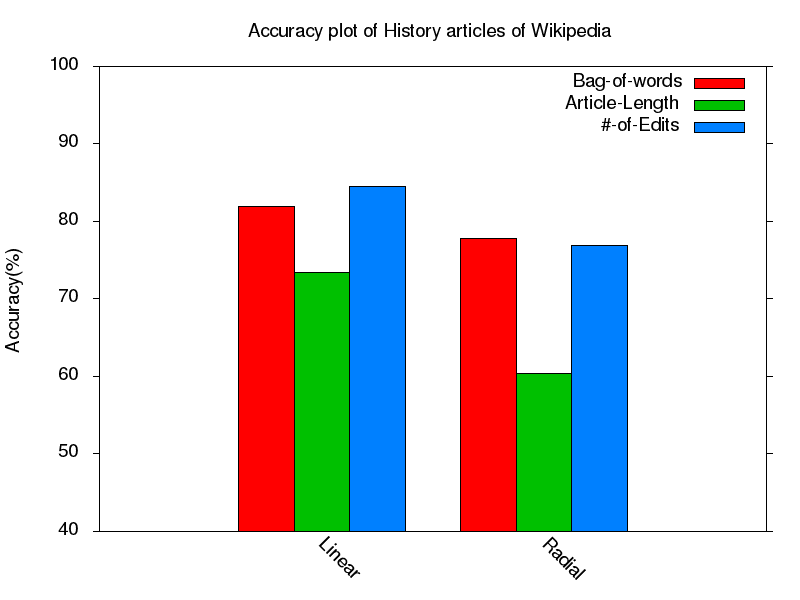
\includegraphics[width=0.95\columnwidth]{accuracy_plot.png}
         \caption{Accuracy on svm classifier with different features}
         \label{fig:block}
 \end{figure}
 \begin{figure}[Politics/Economics]
         \centering
         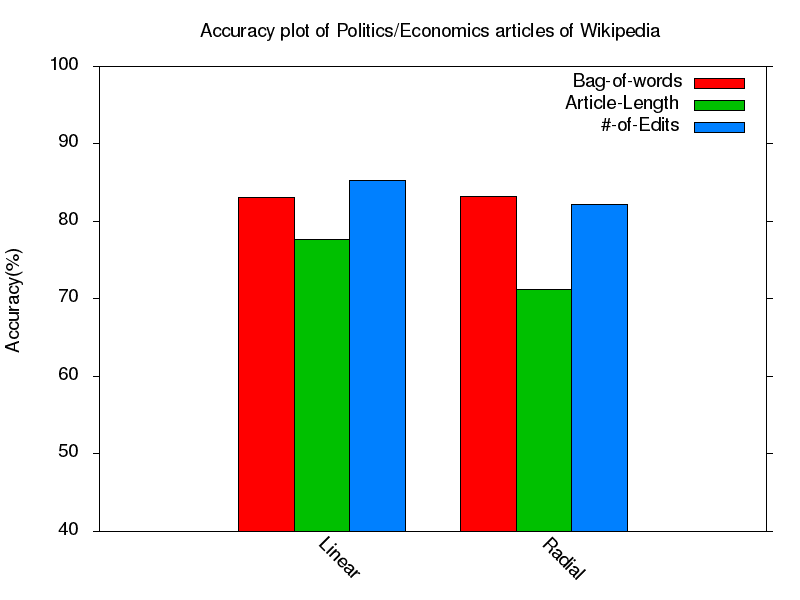
\includegraphics[width=0.95\columnwidth]{accuracy_plot2.png}
         \caption{Accuracy on svm classifier with different features}
         \label{fig:block}
 \end{figure}
 \comment {
 \begin{figure}[Religion]
         \centering
         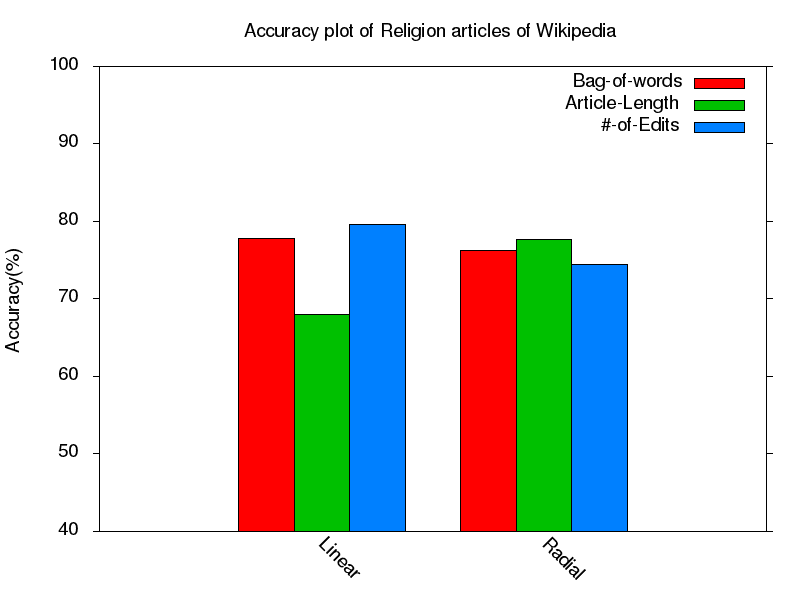
\includegraphics[width=0.95\columnwidth]{accuracy_plot3.png}
         \caption{Accuracy on svm classifier with different features}
         \label{fig:block}
 \end{figure}
 }
 
 \begin{table}[t]
 	\centering
 	\begin{tabular}{|c|c|c|c|c|c|c|c|}
 		\hline
 		\textbf{Class} & \textbf{TP Rate} & \textbf{FP Rate} & \textbf{Precision} & \textbf{Recall} & \textbf{F-measure} & \textbf{MCC} & \textbf{ROC Area} \\
 		\hline
 		\hline
 		Controversial & 0.737 & 0.091 & 0.829 & 0.737 & 0.78 & 0.664 & 0.823 \\
 		Non-Controversial & 0.909 & 0.263 & 0.853 & 0.909 & 0.88 & 0.664 & 0.823\\
 		Weighted Average & 0.845 & 0.199 & 0.844 & 0.845 & 0.843 & 0.664 & 0.823 \\
 		\hline
 	\end{tabular}
 	\centering
 	\caption{SVM Classifier with linear kernel and edit-history-count feature for History category}
 	\label{tab:results}
 \end{table}
 
 \begin{table}[History]
 	\centering
 	\begin{tabular}{|c|c|c|}
 		\hline
 		\textbf{Actual/Predicted} & Controversial &Non-controversial \\
 		\hline
 		Controversial & 87 & 31\\
 		Non-controversial & 18 & 180\\
 		\hline
 	\end{tabular}
 	\caption{Confusion matrix for Linear SVM with edit-history-count as feature for History category}
 	\label{tab:results}
 \end{table} 
 
 
 
 \begin{table}[Politics/Economics]
 	\centering
 	\begin{tabular}{|c|c|c|c|c|c|c|c|}
 		\hline
 		\textbf{Class} & \textbf{TP Rate} & \textbf{FP Rate} & \textbf{Precision} & \textbf{Recall} & \textbf{F-measure} & \textbf{MCC} & \textbf{ROC Area} \\
 		\hline
 		\hline
 		Controversial & 0.695 & 0.082 & 0.777 & 0.695 & 0.734 & 0.634 & 0.806 \\
 		Non-Controversial & 0.918 & 0.305 & 0.879 & 0.918 & 0.898 & 0.634 & 0.806\\
 		Weighted Average & 0.853 & 0.24 & 0.849 & 0.853 & 0.85 & 0.634 & 0.806 \\
 		\hline
 	\end{tabular}
 	\centering
 	\caption{SVM Classifier with linear kernel and edit-history-count feature for Politics/Economics category}
 	\label{tab:results}
 \end{table}
 
 \begin{table}[Politics/Economics]
 	\centering
 	\begin{tabular}{|c|c|c|}
 		\hline
 		\textbf{Actual/Predicted} & Controversial &Non-controversial \\
 		\hline
 		Controversial & 139 & 61\\
 		Non-controversial & 40 & 445\\
 		\hline
 	\end{tabular}
 	\caption{Confusion matrix for Linear SVM with edit-history-count as feature for Politics/Economics category}
 	\label{tab:results}
 \end{table}
 
 \comment {
 \begin{table}[Religion]
 	\centering
 	\begin{tabular}{|c|c|c|c|c|c|c|c|}
 		\hline
 		\textbf{Class} & \textbf{TP Rate} & \textbf{FP Rate} & \textbf{Precision} & \textbf{Recall} & \textbf{F-measure} & \textbf{MCC} & \textbf{ROC Area} \\
 		\hline
 		\hline
 		Controversial & 0.526 & 0.116 & 0.595 & 0.526 & 0.559 & 0.428 & 0.705 \\
 		Non-Controversial & 0.884 & 0.474 & 0.851 & 0.884 & 0.867 & 0.428 & 0.705\\
 		Weighted Average & 0.796 & 0.386 & 0.789 & 0.796 & 0.791 & 0.428 & 0.705 \\
 		\hline
 	\end{tabular}
 	\centering
 	\caption{SVM Classifier with linear kernel and edit-history-count feature for Religion category}
 	\label{tab:results}
 \end{table}
 
 \begin{table}[Religion]
 	\centering
 	\begin{tabular}{|c|c|c|}
 		\hline
 		\textbf{Actual/Predicted} & Controversial &Non-controversial \\
 		\hline
 		Controversial & 139 & 61\\
 		Non-controversial & 40 & 445\\
 		\hline
 	\end{tabular}
 	\caption{Confusion matrix for Linear SVM with edit-history-count as feature for Religion category}
 	\label{tab:results}
 \end{table}
 }
 \comment{

 \begin{table}[t]
         \centering
         \begin{tabular}{|c||cc|}
                 \hline
                 Header 1 & Desc 1 & Desc 2 \\
                 \hline
                 \hline
                 Row 1 & Data 1-1 & Data 1-2 \\
                 Row 2 & Data 2-1 & Data 2-2 \\
                 \hline
         \end{tabular}
         \caption{Table of results.}
         \label{tab:results}
 \end{table}

 And refer as Table \ref{tab:results}.

 }

 \section{Conclusions}

 Clearly state the conclusions.

 Also, outline the future work.


 \bibliographystyle{plain}
 \bibliography{refs}

 \end{document}
